\documentclass[a4paper,12pt]{article} 

%%% Работа с русским языком
\usepackage{cmap}                           % поиск в PDF
\usepackage{mathtext} 			 	       % русские буквы в формулах
\usepackage[T2A]{fontenc}               % кодировка
\usepackage[utf8]{inputenc}              % кодировка исходного текста
\usepackage[english,russian]{babel}  % локализация и переносы
\usepackage[left=2cm,right=2cm,
    top=2cm,bottom=3cm,bindingoffset=0cm]{geometry}
\usepackage{wrapfig}
\usepackage{gensymb}
\usepackage{textcomp}
\usepackage{multirow}
\usepackage{amsmath,amsfonts,amssymb,amsthm,mathtools} % AMS
\usepackage{euscript}	 % Шрифт Евклид
\usepackage{mathrsfs} % Красивый матшрифт
\usepackage{graphicx}%Вставка картинок правильная
\usepackage{float}%"Плавающие" картинки
\usepackage{wrapfig}%Обтекание фигур (таблиц, картинок и прочего)
\title{Лабораторная работа 3.4.5

Петля гистерезиса}
\author{Кагарманов Радмир Б01-106}
\date{14 ноября 2022 г.}

\begin{document}
\maketitle
\thispagestyle{empty}
\newpage
\setcounter{page}{1}

\paragraph{Цель работы:} при помощи осциоллографа исследовать предельные петли гистерезиса и начальные кривые намагничивания для нескольких ферромагнитных образцов; определить магнитные характеристики материалов, чувствительность каналов $X$ и $Y$ осциоллографа и постоянную времени $\tau$ интегрирующей цепочки.

\paragraph{В работе используются:} автотрансформатор, понижающий трансформатор, интегрирующая ячейка, амперметр и вольтметр(мультиметры), резистор, делитель напряжения, электронный осциоллограф, тороидальные образцы с двумя обмотками.

\paragraph{Теория\\} 
К ферромагнетикам принадлежат железо, никель, кобальт, гадолиний, их многочисленные сплавы с другими металлами. К ним примыкают ферриты - диэлектрики со структурой антиферромагнетика.\par
Магнитная индукция $B$ и напряжённость магнитного поля $H$ в ферромагнитном материале неоднозначно связаны между собой: индукция зависит не только от напряжённости, но и от предыстории образца. Связь между индукцией и напряжённостью поля типичного ферромагнетика иллюстрирует рис. 1.
\begin{figure}[!h]
\centering
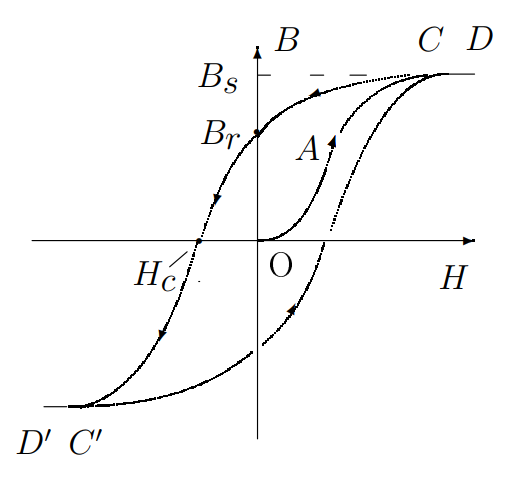
\includegraphics[width=0.5\linewidth]{петля гистерезиса.png}
\caption{Петля гистерезиса}
\label{fig:mpr}
\end{figure}

\paragraph{Экспериментальная установка\\}
Схема установки представлена на рис. 2. Напряжение от сети (220 В, 50 Гц) с помощью трансформаторного блока T, состоящего из регулировочного автотрансформатора (или реостата $R_1$, включённого как потенциометр), подаётся на намагниченную обмотку $N_0$ исследуемого образца.\par
В цепь намагничивающей катушки, на которую подаётся напряжение $U_0 = 6,3~В$, последовательно включены амперметр A и резистор с сопротивлением $R_0$.\par 
Напряжение на $R_0$, равное $U_R = R_0 I_0$, подаётся на канал Х электронного осциоллографа(ЭО). Связь между напряжённостью $H$ в образце и током $I_0$ рассчитываются по теореме о циркуляции.\par
\newpage
\begin{figure}[!h]
\centering
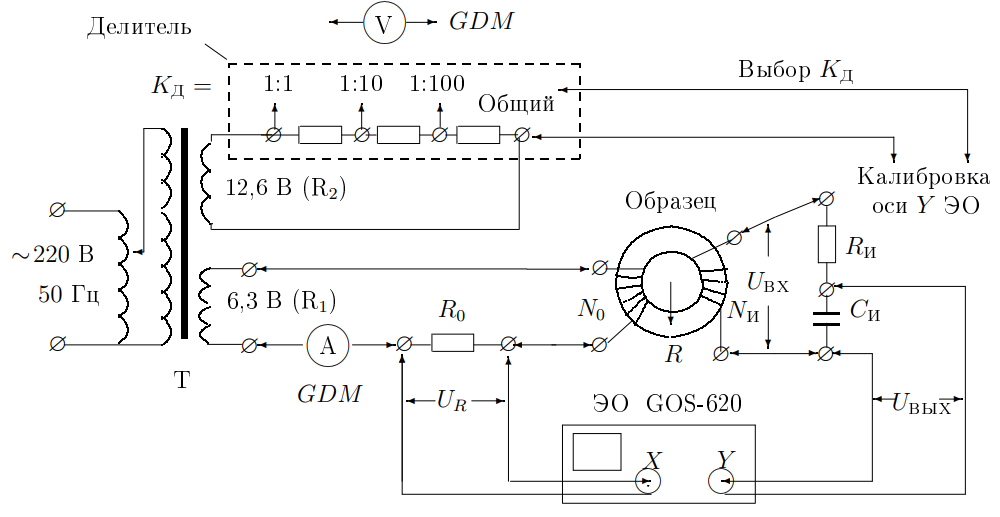
\includegraphics[width=0.9\linewidth]{установка.png}
\caption{Петля гистерезиса}
\label{fig:mpr}
\end{figure}
Для измерения магнитной индукции $B$ с измерительной обмотки $N_и$ на вход интегрирующей $RC$-цепочки подаётся входное напряжение $U_и=U_{вх}$, пропорциональное производной $dB/dt$, а с выхода цепочки снимается напряжение $U_с = U_{вых}$, пропорциональное величине $B$, и подаётся на канал Y ЭО. Значение индукции поля $B$ рассчитывается по формуле:
\begin{equation}
    |B|=\frac{\tau_и}{SN}U_{вых},
\end{equation}
где $\tau_и = R_и C_и$ - постоянная времени $RC$-цепочки. $SN$ - площадь и количество витков.\par
Постоянную времени $RC$-цепочки можно определить экспериментально. С обмотки 6,3 В на вход интегрирующей цепочки подаётся синусоидальное напряжение $U_{вх}$ с частотой $\nu = \omega/2\pi=50$ Гц. На канал Y ЭО или на цифровой вольтметр поочерёдно подаются сигнала со входа ($U_{вх}$) и выхода ($U_{вых}$) $RC$-цепочки. Измерив амплитуды этих сигналов, можно рассчитать постоянную времени по формуле:
\begin{equation}
    \tau = RC = \frac{U_{вх}}{\omega U_{вых}}
\end{equation}

\paragraph{Обработка результатов\\}
\subparagraph{1.}Посчитаем коэффициенты преобразования отклонений по осям ЭО в напряжённость и индукцию.
\begin{equation}
    H=\frac{IN_0}{2\pi R}
\end{equation}
\begin{equation}
    B=\frac{R_и C_и}{SN_и}U_{вых}
\end{equation}
Получаем:
\begin{center}
Кремнистое железо: $k_{H} = 350$, $k_{B} = 9,52$.\\
Феррит 1000нн: $k_{H} = 140$, $k_{B} = 3,33$.\\
Пермаллой: $k_{H} = 145,8$, $k_{B} = 4,78$.
\end{center}


\subparagraph{2.} Для каждого образца рассчитаем коэрцитивное поле $H_c$ и остаточную индукцию $B_r$.
\begin{center}
    Кремнистое железо:  $H_c = 32,6 ~ \frac{А}{м}, B_r = 0,90~ Тл$.
    Феррит 1000нн: $H_c = 4,4 ~ \frac{А}{м}, B_r = 0,33~ Тл$.
    Пермоллoй: $H_c = 19,6 ~ \frac{А}{м}, B_r = 0,81~ Тл$.
\end{center}
\subparagraph{3.}По начальным кривым намагничивания оценим начальные и максимальные значения дифференциальной магнитной проницаемости $\mu_{диф}=dB/dH$.\par
Занесём все результаты в таблицу, для некоторых величин будет записано табличное значение в скобочках.
\begin{center}
\begin{tabular}{|c|c|c|c|}
\hline
Амплит. & Fe-Ni & Fe-Si & Феррит \\ \hline
$H_c, \frac{А}{м}$ & 19,6(4) & 32,6(40) & 4,4(4-100) \\ \hline
$B_s,~ Тл$ & 0,81(1,05) & 0,90(1,95) & 0,33(0,3-0,4) \\ \hline
$\mu_{нач}$ & - & - & - \\ \hline
$\mu_{макс}$ & 21 & 4  & -\\ \hline
\end{tabular}\\
\end{center}
\paragraph{Вывод:}в данной лабораторной работе мы исследовали предельные петли гистерезиса для трёх образцов, определили магнитные характеристики этих образцов, проверили чувствительность каналов осциоллографа.
\end{document}
